\documentclass[11pt]{article}
\input{style/bigdata.txt}
\usepackage{amsmath,amsfonts,amssymb,amsthm,latexsym,graphicx,array,multicol}

% chktex-file 8
% chktex-file 44

\emergencystretch=5mm
\tolerance=400
\allowdisplaybreaks[4]

\theoremstyle{plain}
\newtheorem{theorem}{Theorem}[section]
\newtheorem{proposition}[theorem]{Proposition}
\newtheorem{corollary}[theorem]{Corollary}
\newtheorem{lemma}[theorem]{Lemma}
\newtheorem{problem}[theorem]{Problem}

\theoremstyle{definition}
\newtheorem*{remark}{Remark}

\title{GOA-KNN:\@ Electronic Annotation of Gene Ontology Terms}
\author{Daniel Syomichev}

\newcommand{\Programme}{Data Science and Analytics}

\begin{document}
\maketitle

\declaration{}

\begin{abstract}
\end{abstract}

\section{Introduction}\label{sec:introduction}

The primary goal of this project is to provide a tool which, given an arbitrary biomedical text, returns a ranked list of Gene Ontology (GO)~\cite{ashburner/2000/gene,consortium/2025/gene} terms that characterize the text. This project is intended as a direct substitute to the GOCat program by Gobeill et al.\ \cite{gobeill/2013/managing}, and functions on the identical premise that GO terms already attributed to a biomedical text can be used to infer the annotations of a new text through the use of the $K$ nearest neighbors (KNN) algorithm.

\subsection{The Gene Ontology}\label{sec:introduction-ontology}

The Gene Ontology (GO)~\cite{consortium/2025/gene} is a hierarchical vocabulary aimed at categorizing and standardizing biological terminology, particularly with regard to the properties of gene products. The motivation behind the GO `is to produce a dynamic, controlled vocabulary' which is applicable even as the knowledge base changes~\cite{ashburner/2000/gene}. Structurally, it is a set of Directed Acyclic Graphs (DAG), with specificity increasing proportionally with distance from the root node; a node represents a term, with relations represented by edges of the graph.

Each of the three roots, referred to officially as \textit{aspects}, represent different elements of a gene process: Molecular Function, Cellular Component, and Biological Process. No term appears in more than one aspect, but relations may reference terms contained in different aspects.

\subsection{Biomedical Annotations}\label{sec:introduction-annotations}

The immense quantity of available biomedical literature creates significant difficulties in efficiently searching and parsing relevant information. This has led to the widespread adoption of tools which are capable of classifying documents and extracting valuable information from them~\cite{hunter/2006/biomedical}.  An annotation is an assertion between a gene product and terms within an ontology~\cite{hill/2008/gene}, and manual curation of annotations is a time-consuming task. Automatic or electronic annotations are commonly used to provide a `large number of high-quality functional annotations across a broad taxonomic range'~\cite{huntley/2014/database}. For many species, they are the sole source of annotations available~\cite{huntley/2014/database}.

The Gene Ontology Annotation (GOA) project from the European Bioinformatics Institute~\cite{huntley/2014/database} aggregates annotations into a singular point of reference, combining both manual annotations from the Gene Ontology Consortium (GOC) and a total of nine electronic annotation pipelines. Most annotations in the dataset contain a literature reference which supports the existence of the annotation~\cite{hill/2008/gene}. Informally, the GOA dataset can thus be considered as a mapping from a specific publication to a GO term by exploiting this property of the dataset.

\subsection{GOCat}\label{sec:introduction-gocat}

Early approaches to electronic annotation of GO terms were thesaurus or dictionary based, utilizing lexical matching of GO term descriptors and synonyms and the input text. This methodology is limited by the representation of a term within text, where it does not often match to the highly precise label within the ontology~\cite{gobeill/2013/managing}. The GOCat tool was developed by Gobeill et al.\ at the University of Geneva~\cite{gobeill/2013/managing} in order to address this limitation of dictionary-based approaches. The tool compared an arbitrary input text against a corpus of annotated publication abstracts indexed using the Terrier Platform~\cite{ounis/2006/terrier}. Results were scored using the BM25 algorithm~\cite{amati/2009/bm}, and the annotated terms of the highest-scoring neighbors were collected and weighed according to similarity. The aggregate scores were then sorted to yield the final ranked prediction. Using the mean reciprocal rank (MRR) as a precision metric and the macro average recall (MAR), the KNN approach consistently outperformed the dictionary-based method.

\subsection{Aims and Motivation}\label{sec:introduction-aims}

The program corresponding to this project is composed of two abstracted primary components. The vectorizer, which encodes raw text documents into a real vector space, and the classifier, which compares a test input to a fully vectorized collection of document in order to assign the most applicable GO terms to it. Importantly, these components are defined by their function rather than implementation, as the goal is to design them in a modular fashion such that it is possible to examine the differences between different implementations. This project utilizes this design philosophy to compare two vectorization methods and evaluate the effectiveness of each.

The motivation behind this project is simple, GOCat is no longer officially available. This serves as the primary analytical entry-point, since the quantity of both biomedical text and annotations linking publications to GO terms has substantially increased, and the high availability of pre-trained language models provides an alternative vectorization method to evaluate. The representation of a document is treated as in independent parameter within the experiment, allowing direct comparisons between vectorization methods. In place of the Terrier Platform, this project utilizes a term and inverse document frequency sparse vector representation, and additionally implements a dense representation using contextual embeddings produced by the BiomedBERT model~\cite{gu/2021/domainspecific}.

\subsection{Glossary and Notation}\label{sec:introduction-glossary}

Presented below is a glossary which describes the phrasing and terminology used throughout this report. In order disambiguate certain concepts, alternate words are utilized to represent different concepts with similar or same naming schemes.

\begin{table}\label{tab:terminology}
    \centering
    \begin{tabular}{| m{10em}  |m{20em} |}
        \hline
        Phrase        & Description                                                \\
        \hline
        \hline
        term          & References specifically a GO term.                         \\
        \hline
        token         & Used to differentiate GO terms from other types of terms.  \\
        \hline
        document      & A biomedical publication abstract.                         \\
        \hline
        corpus        & A collection of document.                                  \\
        \hline
        vectorization & A vector representation of a document.                     \\
        \hline
        vectorizer    & An object which translates documents into  vectorizations. \\
        \hline
        index         & A collection of vectorizations based on a corpus.          \\
        \hline
        indexing      & The process of vectorizing a corpus.                       \\
        \hline
    \end{tabular}
\end{table}

Certain abbreviations and acronyms are frequently utilized within this report, and the following table lists them alongside the phrase they represent.

\begin{table}\label{tab:abbreviations}
    \centering
    \begin{tabular}{| m{5em} | m{25em} |}
        \hline
        Acronym & Phrase                                                  \\
        \hline
        \hline
        GO      & Gene Ontology                                           \\
        \hline
        GOC     & Gene Ontology Consortium                                \\
        \hline
        GOA     & Gene Ontology Annotations                               \\
        \hline
        TF      & Term Frequency                                          \\
        \hline
        IDF     & Inverse Document Frequency                              \\
        \hline
        BERT    & Bidirectional Encoder Representations from Transformers \\
        \hline
        KNN     & $K$ Nearest Neighbors                                   \\
        \hline
        OEC     & Output Embedding Centering                              \\
        \hline
        MRR     & Mean Reciprocal Rank                                    \\
        \hline
        MAR     & Macro-average Recall                                    \\
        \hline
        HP      & Hierarchical Precision                                  \\
        \hline
        HR      & Hierarchical Recall                                     \\
        \hline
        HF      & Hierarchical F-score                                    \\
        \hline
        GOID    & Gene Ontology Identifier                                \\
        \hline
        PMID    & PubMed Identifier                                       \\
        \hline
    \end{tabular}
\end{table}

\section{Background Research}\label{sec:background}

This section provides a detailed overview of the concepts used throughout the project, as well as summarize each concepts specific use case within the program.

\subsection{Lexical Vectorization (TF-IDF)}\label{sec:background-lexical}

The classifier used in this project is modeled after GOCat~\cite{gobeill/2013/managing}, in which Gobiell et al.\ utilized what was in practice a KNN algorithm alongside a score aggregation function to provide predictions. Much of this functionality was provided by the Terrier platform~\cite{ounis/2006/terrier}, which makes available a number of advanced indexing and retrieval techniques, and was deemed too heavy for use within this project.

By it's nature, the KNN algorithm compares vectors in a $p$-dimensional space and selects the $K$ nearest points based on a predefined distance metric. But documents are not points and cannot be directly compared using the KNN algorithm. They must first be encoded into that $p$-dimensional vector space such that the desired distance metric can also be defined. Within this project this task is achieved in two ways, the first of which is using the term frequency -- inverse document frequency (TF-IDF) method.

\subsubsection{Tokenization Strategies}\label{sec:background-lexical-tokenization}

An extension of the bag-of-words method~\cite{kim/2019/multicotraining}, TF-IDF  is dependent on the decomposition of raw text into ordered sequences of tokens, referred to here as tokenization. The TF-IDF process makes no distinction regarding the definition of a token, and the specific construction of a token is largely defined by the tokenization strategy in place. The TF-IDF process simply takes into account the frequencies of tokens within a document and the corpus as a whole.

The specific tokenization strategy employed by Gobeill et al.\ with GOCat~\cite{gobeill/2013/managing}, and extended within this project, can be condensed into three steps. First, the raw text is decomposed into an ordered sequence of words. This includes the removal of whitespace, punctuation, and numeric sequences of characters. The sequence is then filtered against a list of the most common English language words, known as stop words. Finally, each word in the filtered sequence is reduced to it's root form, in a process known as Porter stemming~\cite{porter/1980/algorithm}. This unifies differing forms of words carrying similar semantic meaning under one subword. For example, the words \textit{biology} and \textit{biological} are both reduced to the root form \textit{biolog}.

It must be noted that the TF-IDF process follows that of tokenization, not the other way around. The importance of a good tokenization strategy will become evident once the TF-IDF process has been described in Section~\ref{sec:background-lexical-weighting}, and will be discussed further in Section~\ref{sec:background-lexical-encoding}.

\subsubsection{Token Weighting}\label{sec:background-lexical-weighting}

Let $D$  be a set of documents constituting a corpus, where each document is represented by an ordered sequence of tokens $d = (t_1, t_2, t_3, \dots)$.

\begin{multicols}{2}
    \begin{equation}\label{eq:tf}
        \operatorname{tf}_{t,d} = \sum_{t_i\in d} 1[t_i = t]
    \end{equation}
    \break{}
    \begin{equation}\label{eq:df}
        \operatorname{df}_{t, D} = \sum_{d\in D} 1[t \in d]
    \end{equation}
\end{multicols}

Equation~\ref{eq:tf} represents the token frequency (TF), the number of times a token appears within a document. Equation~\ref{eq:df} represents the document frequency (DF), the number of documents in the corpus in which a token appears at least once~\cite{manning/2008/scoring}. The inverse document frequency (IDF), first described by in 1972 by Jones~\cite{jones/1972/statistical}, is an extension of Equation~\ref{eq:df} and defined in Equation~\ref{eq:idf} using the definition detailed by Manning et al.\ \cite{manning/2008/scoring}.

\begin{equation}\label{eq:idf}
    \operatorname{idf}_{t, D} = \log{\frac{|D|}{\operatorname{df}_{t, D}}}
\end{equation}

The IDF assigns a weight to a token which logarithmically shrinks as the document frequency grows, such that a common token receives a lower weight. By putting Equations~\ref{eq:tf} and~\ref{eq:idf} together, the final TF-IDF score for a token is defined in Equation~\ref{eq:tfidf}.

\begin{equation}\label{eq:tfidf}
    \operatorname{Score}(t, d, D) = \operatorname{tf}_{t,d} \cdot \operatorname{idf}_{t, D}
\end{equation}

Each token's score can therefore be considered as the quality of differentiation between documents that the token provides. Adapting the description from Robertson~\cite{robertson/2004/understanding}, a token which appears in many documents, for example \textit{protein} across the corpus tested in this project, is not a good differentiator of documents and should be assigned a lower score than an uncommon token such as \textit{deoxyglucopyranosid}.

\subsubsection{Sparse Encoding}\label{sec:background-lexical-encoding}

Define the vocabulary of a corpus to be $V_D$, which is the set of all distinct tokens appearing within the corpus. Let $p=|V_D|$, and define a fixed ordering of tokens with the vocabulary as $V'_D = (v_1, \dots, v_p)$, such that each token corresponds to a particular feature of the $p$-dimensional vector space. A document can then be encoded into its vector representation, the process for which is defined in Equation~\ref{eq:sparse-vector}.

\begin{equation}\label{eq:sparse-vector}
    x_d = (\operatorname{Score}(v_1,d,D), \dots , \operatorname{Score}(v_p,d,D)) \in \mathbb{R}^p
\end{equation}

The key property of this transformation to note is that the score is computed against each token in the vocabulary, not the document. Any token not appearing in the document receives a score of zero, meaning for a vocabulary of significant size and variety, the vector representation will be mostly composed of features with a value of zero, also known as a sparse vector.

As evidenced by the construction of the document vectorization in Equation~\ref{eq:sparse-vector}, the tokenization process is a large factor in the success or failure of TF-IDF vectorization. The tokens selected to be a part of the vocabulary play a large role in ensuring the vectorization is an accurate representation of the document throughout the corpus. Leaving too many common tokens results in document vectors which are indistinguishable from one another, while stripping too many away results in a document vector which is so specific to the particular document, it cannot be grouped with other documents in the corpus. This is in essence a partitioning optimization, where the optimal ratio of specificity must be found in order for the vectorization to be representative of the document not only independently, but also as part of the overarching corpus.

\subsection{Contextual Vectorization (BERT)}\label{sec:background-contextual}

Language models, such as the Bidirectional Encoder Representations from Transformers (BERT)~\cite{devlin/2018/bert}, provide the second vectorization method alluded to in Section~\ref{sec:background-lexical}. The BERT family of language models, first introduced by Devlin et al.\ \cite{devlin/2018/bert} in 2018 provide a framework to contextualize the information encoded throughout an input sequence~\cite{jurafsky/2026/speech}, essentially encoding a document through it's context as opposed to it's lexicographic properties. Vitally, the contextualized output of the model is presented as a a sequence of vectors in real space, which is exactly the format the KNN algorithm expects.

\subsubsection{Embeddings}\label{sec:background-contextual-embeddings}

Mirroring the TF-IDF process described in Section~\ref{sec:background-lexical}, vectorization utilizing a BERT model also requires a tokenization step, here handled by the WordPiece algorithm developed by Wu et al.\ \cite{wu/2016/googles}. Perhaps the most important difference between this algorithm and the strategy described in Section~\ref{sec:background-lexical-tokenization} is that the WordPiece algorithm utilizes a fixed vocabulary of word fragments, also known as subwords. The input text is recursively split on the longest subword within the vocabulary, and any portions of the input which are not represented in the vocabulary are replaced by a designated token representing unknown character sequences. The fixed vocabulary size means there is no dependence on the corpus as seen in the TF-IDF process and described in Section~\ref{sec:background-lexical-encoding}.

The resulting sequence of tokens is then encoded as an input embedding, the sum of the token identity, segment and positional embeddings~\cite{devlin/2018/bert}. These three embeddings are learned during the model's pretraining, and the resulting input embedding is at this point dependent only it's own identity and position in the input sequence~\cite{kubek/2025/selfimproving, huang/2021/multiplicative}. The input embeddings, true to their name, serve as the input to the model, which then passes them through it's layers to finally result in output embeddings, which have been contextualized. The BERT model architecture uses bidirectional self-attention, first presented by~\cite{vaswani/2017/attention}, which Devlin et al.\ describe to be property that each token is capable of attending to the context across the entire input sequence~\cite{devlin/2018/bert}. This ensures that each token's output embedding is reflection of the token's context within the entire input, meaning two instances of the same token in different documents have different output embeddings. This property is the clear differentiator between this method and the TF-IDF vectorization described in Section~\ref{sec:background-lexical-encoding}. Where TF-IDF only considers the distribution of tokens within a document, contextual embeddings additionally consider the context in which those tokens exist.

\subsubsection{Mean Pooling}\label{sec:background-contextual-pooling}

Alongside the sequence of tokens, the tokenization step described in Section~\ref{sec:background-contextual-embeddings} also constructs an attention mask, a sequence $a=(a_1, a_2,a_3,\dots)$ where $a_i \in \{0,1\}$. This identifies the positions within the sequence which are not representative of the input, such as padding token positions.

The model outputs one embedding per token, which necessitates a pooling strategy in order to provide the per document representation required by the KNN algorithm. The mean-pooling strategy, described by Tang et al.\ to be the average taken over the output embeddings~\cite{tang/2024/pooling}, is a strategy which does not involve additional training and is applicable to the bidirectional self-attention architecture of the BERT model. This must be taken with respect to the attention mask, as the model still outputs an embedding for the non-representative padding tokens. With the sequence of output embeddings $e=(e_1, e_2, e_3, \dots)$ the document's contextual vectorization is defined in Equation~\ref{eq:dense-vector}.

\begin{equation}\label{eq:dense-vector}
    z_d = \frac{\sum_{i} {e_i}{a_i}}{\sum_{i} a_i}
\end{equation}

This results in a dense vector in $\mathbb{R}^{768}$ which is entirely independent of the corpus, unlike the vectorization described in Section~\ref{sec:background-lexical-encoding}.

\subsubsection{Domain Specific Pretraining}\label{sec:background-contextual-domain}

There exist two distinct methods to pretraining a domain specialized BERT model: mixed domain and domain specific. Mixed domain pretraining essentially initializes the original BERT model, which was pretrained on Wikipedia and BookCorpus~\cite{devlin/2018/bert}, and continues the pretraining process on in-domain text. Domain specific instead trains the model from scratch using only the in-domain text~\cite{gu/2021/domainspecific}.  Gu et al.\ found that domain specific pretraining significantly outperformed mixed domain pretrained model, particularly in domains with an abundance of available literature~\cite{gu/2021/domainspecific}.

Given the domain specific context of this project, this result is particularly important in selecting a specific BERT variant to drive the vectorization process. As such, the model chosen as the default for this project was BiomedBERT~\cite{gu/2021/domainspecific}, a model trained from scratch by Gu et al.\ on biomedical abstracts from PubMed and full text articles from PubMedCentral~\cite{sayers/2024/database}. This is the ideal candidate in that the documents being indexed in this project are also biomedical abstracts sourced from PubMed.

\subsubsection{The Anisotropic Phenomenon}\label{sec:background-contextual-anisotropy}

After implementation of the BERT vectorization method, it was observed that the distances returned by the KNN algorithm all appeared within an incredibly small range. This made it difficult for the scoring function, described later in Section~\ref{sec:methods-scoring} to effectively aggregate the scores and provide a valid result. After subsequent research it was determined that this was not a peculiarity of the data, but rather a well document property of the BERT architecture called the anisotropic phenomenon.

First described by Gao et al.~\cite{gao/2019/representation}, the problem of anisotropy refers to the uneven distribution of contextual embeddings within a the vector space. Geometrically, the vectors are not distributed uniformly within the vector space, instead occupying a narrow cone~\cite{ethayarajh/2019/contextual}. Using direction-based similarity metrics then results in a positive correlation between any two unrelated words~\cite{gao/2019/representation}. Ethayarajh also showed that the anisotropy of embeddings grows with each consecutive model layer~\cite{ethayarajh/2019/contextual}. The actual result of this phenomenon is displayed in Figure~\ref{fig:contextual-dim1-vs-dim2}, which plots the first two dimensions of the document vectorizations produced using the contextual vectorization method.

\begin{figure}\label{fig:contextual-dim1-vs-dim2}
    \centering
    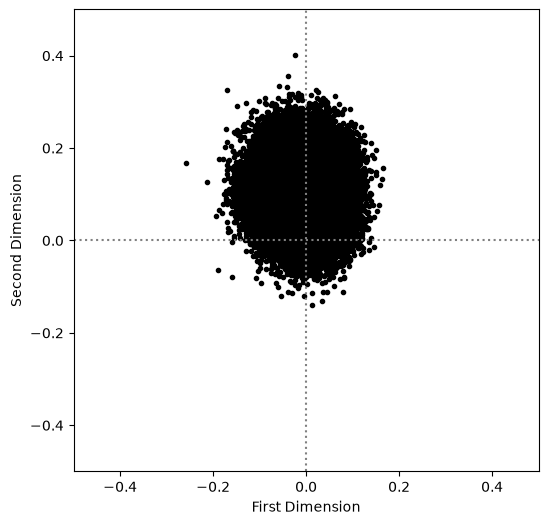
\includegraphics[width=0.75\linewidth]{figures/embedding_d1_d2.png}
    \caption{First two dimensions of document vectorizations produced with BERT vectorization method.}
\end{figure}

There is a noticeable shift away from the origin in the first two dimensions, such that direction based comparison techniques, such as the cosine distance metric used in this project, struggle. Stollenwerk et al.\ propose a mitigation strategy they describe as output embedding center (OEC), which involves centering the mean output embedding at the origin~\cite{stollenwerk/2026/output}. This is done by subtracting the mean output embedding from each output embedding, effectively normalizing the magnitude around zero. Biś et al.\ found that output embeddings tend to be isotropic around their center~\cite{bis/2021/much}, suggesting the mean centering strategy restores the isotropic property necessary for direction-based comparison. Figure~\ref{fig:contextual-dim1-vs-dim2-scaled} shows the effect on the first two dimensions of the document vectorizations after applying the mean centering technique.

\begin{figure}\label{fig:contextual-dim1-vs-dim2-scaled}
    \centering
    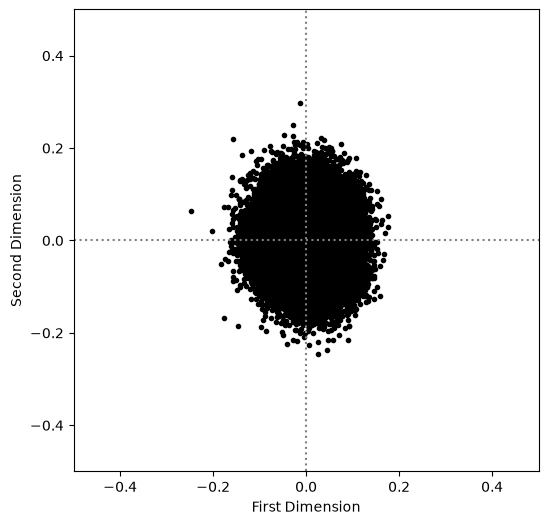
\includegraphics[width=0.75\linewidth]{figures/embeddings_d1_d2_scaled.png}
    \caption{The first two dimensions of document vectorizations after applying mean centering.}
\end{figure}

\subsection{Measuring Distance}\label{sec:distance}

A key component of the KNN algorithm, and by extension the classifier alluded to in Section~\ref{sec:introduction-aims}, is the distance metric used to compare the vectorizations produced by the methods described in Sections~\ref{sec:background-lexical-encoding} and~\ref{sec:background-contextual-embeddings}. Given that the an important goal of the project is to compare these two methods, the distance metric used in the classifier should be a fixed parameter. These methods emit vectors of very different constructions, and the distance metric must be equally meaningful for both.

In order to disqualify the standard candidate, Euclidean Distance, it is prudent to first define it. Let two vectors $a, b \in \mathbb{R}^{n}$ such that $a = (a_1, \dots, a_n)$ and $b = (b_1, \dots, b_n)$. The Euclidean Distance, expressed in Equation~\ref{eq:euclidean} is the norm of the difference between the two vectors~\cite{lay/2021/linear}.

\begin{equation}\label{eq:euclidean}
    \operatorname{Euclidean\ Distance} = {\Vert a-b \Vert}_2 = \sqrt{{(a_1-b_1)}^2 + \cdots + {(a_n - b_n)}^2} \in \mathbb{R}
\end{equation}

From Equation~\ref{eq:euclidean} it is clear the the magnitude of a vector is primary contributor to the distance, which is an undesirable result for both vectorization methods, but for differing reasons. In the case of sparse vectorization from Equation~\ref{eq:sparse-vector}, the magnitude of a vector grows alongside the raw quantity of tokens a document decomposes into. As a result, two documents utilizing the same language will actually be attributed a distance based on the difference in their length. By contrast, Euclidean distance is a poor metric for the dense embeddings produced by Equation~\ref{eq:dense-vector} due to lack of absolute magnitude. As evidenced by Figure~\ref{fig:contextual-dim1-vs-dim2}, the contextual vectorizations are all clustered around a singular centroid, meaning a magnitude-based distance metric will report low distances between any two vectorizations. Intuitively, the Euclidean distance metric will struggle to report low distances for the TF-IDF vectorization, even if they are semantically similar. For BERT vectorization the problem is opposite, such that all vectorizations will appear to be similar even when they are not.

\begin{equation}\label{eq:cosine-similarity}
    \operatorname{Cosine\ Similarity} = \frac{a \cdot b}{\Vert a \Vert \Vert b \Vert}\ \in [-1, 1]
\end{equation}

The cosine similarity, defined in Equation~\ref{eq:cosine-similarity}~\cite{you/2025/semantics} is the more appropriate metric. It is invariant to magnitude~\cite{you/2025/semantics}, neutralizing the influence of the length and absolute frequency of terms in the document in the case of TF-IDF vectorizations, while also providing a more precise distinction of the BERT vectorizations. The cosine distance, defined in Equation~\ref{eq:cosine-distance}~\cite{you/2025/semantics}, is a simple remapping of cosine similarity to represent higher similarity at lower distance. This is necessary since the KNN algorithm expects closer neighbors to share a smaller distance.

\begin{equation}\label{eq:cosine-distance}
    \operatorname{Cosine\ Distance} = 1 -  \operatorname{Cosine\ Similarity} \in [0, 2]
\end{equation}

\section{Software Development}\label{sec:development}

\section{Methods}\label{sec:methods}

\section{Analysis of Results}\label{sec:analysis}

\subsection{Evaluation Metrics}\label{sec:analysis-metrics}

% TODO: Explain how this relates to the program, and why research needed to be conducted on this.

In order to accurately assess the effectiveness of the classifier presented in Section~\ref{sec:methods-scoring}, it is important to define metrics which are applicable to the label space of the prediction. In the case of GOCat~\cite{gobeill/2013/managing}, as well as the classifier provided by this project, a prediction is a ranked sequence of terms ordered by score emitted by the scoring function, which was additionally truncated to a maximum allowable length. By contrast, the true labels are an unordered, arbitrary length set with no internal ranking scheme. The ontology itself is also hierarchical by construction, implying the possibility of the classifier predicting a child or parent of the true term. These predictions are not wrong in the binary sense, since there is a relationship between the two terms the classifier may have learned. Thus, any metrics used to evaluate the classifier must take at least a subset of these properties into account. Two types of metrics were found to be applicable and are described in the Sections~\ref{sec:analsysis-metrics-exact} and~\ref{sec:analysis-metrics-hierarchical}.

Let $D_{test}$ represent the set of test documents, such that $T_d=\{ t_1, \dots, t_n \}$ is the set of $n$ terms annotated to document $d \in D_{test}$, and $\hat{T}_d=(\hat{t}_1, \dots , \hat{t}_l )$ be the ranked prediction sequence returned by the classifier which has been truncated to a fixed length of $l$.

\subsubsection{Exact Matching}\label{sec:analsysis-metrics-exact}

The first set of metrics treats the label space of terms to be independent of one another, only considering exact matches during evaluation. Used Gobiell et al.\ to evaluate GOCat~\cite{gobeill/2013/managing}, these two metrics represent the model's ability to exactly predict the desired label space, with no consideration for the hierarchical nature of the ontology.

The mean reciprocal rank (MRR), defined in equation~\ref{eq:mrr}, measures the mean position at which the ranked sequence provides a correct prediction across the set of test documents~\cite{radev/2002/evaluating}. Formally, define the rank set of a prediction sequence to be $\hat{R}_d = \{  i : \hat{t}_i \in T_d \}$, such that it contains the rank of each correctly predicted term in $\hat{T}_d$.

\begin{multicols}{2}
    \begin{equation}\label{eq:rr}
        \hat{r}_d =
        \begin{cases}
            0                      & \textnormal{if } |\hat{R}_d| = 0 \\
            {(\min\hat{R}_d)}^{-1} & \textnormal{otherwise}
        \end{cases}
    \end{equation}
    \break{}
    \begin{equation}\label{eq:mrr}
        \operatorname{MRR} = \frac{1}{|D_{test}|} \sum_{d \in D_{test}} \hat{r}_d
    \end{equation}
\end{multicols}

The macro-average recall (MAR), defined in equation~\ref{eq:mar}, measures the per-term proportion of the case that a term was both annotated to a document and predicted to be so. Let $Y_{test} = \bigcup_{d \in D_{test}} T_d$ be the set of all true terms annotated to documents in the test set. Then for each term, define $F_t = \bigcup_{d \in D_{test}} \{d : t \in T_d\}$ and $G_t = \bigcup_{d \in D_{test}} \{d : t \in \hat{T}_d\}$ to be the sets of documents that contain the term $t$ appearing in the true and predicted sets respectively. % TODO: need a non-website citation for this.

\begin{equation}
    \operatorname{MAR} = \frac{1}{|Y_{test}|} \sum_{d \in D_{test}} \frac{|F_t \cap G_t|}{|F_t|}
    \label{eq:mar}
\end{equation}

Importantly, each term contributes equally to the average, so terms which are disproportionally represented within the test set are not given precedence.

\subsubsection{Hierarchical}\label{sec:analysis-metrics-hierarchical}

The deficit of the the metrics defined in Section~\ref{sec:analsysis-metrics-exact} is the lack of consideration for the relationship between terms. A term which sits one level above the expected term scores just as badly as a term which appears in a separate aspect altogether, which invalidates the ontology's structure entirely. Verspoor et al.\ demonstrated that the standard multi-label evaluation metrics of precision, recall and F-score report poor performance due to this lack of consideration~\cite{verspoor/2006/categorization}, and propose extensions to these metrics which take the strength of the relationship between terms into account. Here ${\uparrow} t$ and ${\uparrow} \hat{t}$ represent the lineage expansions of a true and predicted term respectively. In plain words, these are the sets containing a term and all of it's ancestors.

\begin{multicols}{2}
    \begin{equation}\label{eq:hpd}
        \operatorname{hp}_d = \frac{1}{|\hat{T}_d|} \sum_{\hat{t} \in \hat{T}_d} \max_{t \in T_d} \frac{|{\uparrow} t \cap  {\uparrow} \hat{t}|}{|{\uparrow} \hat{t}|}
    \end{equation}
    \break{}
    \begin{equation}\label{eq:hp}
        \operatorname{HP} = \frac{1}{|D_{test}|} \sum_{d \in D_{test}} \operatorname{hp}_d
    \end{equation}
\end{multicols}

\begin{multicols}{2}
    \begin{equation}\label{eq:hrd}
        \operatorname{hr}_d = \frac{1}{|T_d|} \sum_{t \in T_d} \max_{\hat{t} \in \hat{T}_d} \frac{|{\uparrow} t \cap  {\uparrow} \hat{t}|}{|{\uparrow} t|}
    \end{equation}
    \break{}
    \begin{equation}\label{eq:hr}
        \operatorname{HR} = \frac{1}{|D_{test}|} \sum_{d \in D_{test}} \operatorname{hr}_d
    \end{equation}
\end{multicols}

Equations~\ref{eq:hpd} and~\ref{eq:hrd}, are calculated for each document in the test set. Hierarchical precision (HP) and hierarchical recall (HR) are then the average score across all the documents in the test set, as described in Equations~\ref{eq:hp} and~\ref{eq:hr}. Verspoor et al.\ also propose a hierarchical F-score (HF), which is first calculated per document in Equation~\ref{eq:hfd}  as the harmonic mean of the per document hierarchical precision and recall, and then averaged over all documents in the test set in equation~\ref{eq:hf}~\cite{verspoor/2006/categorization}.

\begin{multicols}{2}
    \begin{equation}\label{eq:hfd}
        \operatorname{hf}_d = 2 \frac{\operatorname{hp}_d \cdot \operatorname{hr}_d}{\operatorname{hp}_d + \operatorname{hr}_d}
    \end{equation}
    \break{}
    \begin{equation}\label{eq:hf}
        \operatorname{HF} = \frac{1}{|D_{test}|} \sum_{d \in D_{test}} \operatorname{hf}_d
    \end{equation}
\end{multicols}

For hierarchical precision, this definition makes the several key distinctions which make it suitable for evaluating hierarchical predictions. First, there is an increased penalty for predicting an incorrect general term, as opposed to a specific one. The penalty is also proportional with the distance between a predicted term and nearest expected ancestor~\cite{verspoor/2006/categorization}. The use of the maxima within the equations ensures that each term is only compared against it's closest match, as opposed to an average over all possible terms~\cite{verspoor/2006/categorization}.

Verspoor et al.\ describe the characteristics of the metrics by comparing situations where there is a single prediction and single truth. If the prediction is a descendant of the expected term, then $HR=1$ and $HP<1$. In the opposite situation, where the prediction is an ancestor of the expected term, $HR < 1$ while $HP=1$. Thus a classifier which scores highly on $HR$ and poorly on $HP$ is generally predicting terms which are more specific than expected and vice versa~\cite{verspoor/2006/categorization}.

\subsubsection{Comparability}\label{sec:analysis-metrics-comparability}

Equations~\ref{eq:mrr} (MRR),~\ref{eq:hp} (HP),~\ref{eq:hr} (HR) and~\ref{eq:hf} (HF) are defined per document, and then averaged over the whole test set, while equation~\ref{eq:mar} (MAR) is defined per-term and averaged over all terms in the test set, depicting a fundamental difference in axis for the metrics. As a result, it is inaccurate to compare MAR and HR, despite both representing a form of recall. Additionally, Gobiell et al.\ treated MRR as a precision metric in their tests~\cite{gobeill/2013/managing}, but due to it's construction around rank sensitivity, it cannot be compared to the HP metric either. Lastly, the hierarchical metrics are not comparable to their standard counterparts. Verspoor et al.\ note that `HP and HR will always be higher than the corresponding P and R values for a given test set' and are `not comparable metrics'~\cite{verspoor/2006/categorization}. Aligned with the reasoning stated above, all metrics will be reported independently, and not compared among each other in the following sections. The primary driving force of the analysis is thus the change in these metrics, as opposed to directly comparing them.

\subsection{Hyperparameter Tuning}\label{sec:analsysis-tuning}

\subsection{Head-to-Head Comparison}\label{sec:analsysis-comparison}

\subsection{Temporal Evolution}\label{sec:analsysis-temporal}

\section{Self Assessment}\label{sec:assessment}

\section{User Manual}\label{sec:manual}

\bibliographystyle{plain}
\bibliography{bibliography}

\section{Appendix}\label{sec:appendix}

\end{document}